
\chapter{Vladimir Sierra}



\section{Un poco sobre mí}

Tengo 18 años, me llamo Vladimir, nací y viví hasta los 15 años en TLapa Guerrero.
Durante toda mi vida he sentido gran pasión por las Matemáticas; también me interesan mucho las artes, toco guitarra y piano. Siempre he querido aprender a pintar pero creo que no es algo en lo que sea bueno.
Mis gustos musicales son un poco variados, pero creo que el género que más me deleita escuchar es la trova.
SI pudiera resumir mis gustos diría, que mi músico favorito es SIlvio Rodríguez, escritor favorito es Haruki Murakami, y pintor favorito quizá sea Francisco de Goya.
También me interesa mucho el fútbol, antes solía jugar, pero a partir de que las obligaciones en la escuela se volvieron más pesadas lo deje.
Acabo de ingresar a la Facultad de Ciencias para estudiar Ciencias de la Computación.

Haruki Murakami es de mis autores favoritos, entre mis libros favoritos de él están 

\subsection {hobbies}
\begin{enumerate}
\item Tocar guitarra
\item Jugar soccer
\item Leer
\item Estudiar Matemáticas
\end{enumerate}  

Escogí la carrera porquer: 


\begin{itemize}
\item Me gustan las estructuras
\item Me gusta resolver problemas
  \item Soy bueno en Análisis Matemático
 \end{itemize}

\newpage

    \section{Películas favoritas}
    Mis trilogía favorita es sin duda la del Señor de los anillos, pero algo que tengo pendiente por hacer es leer los libros~\cite{torres,comunidad,retorno}
    
\begin{figure}[h]
\centering
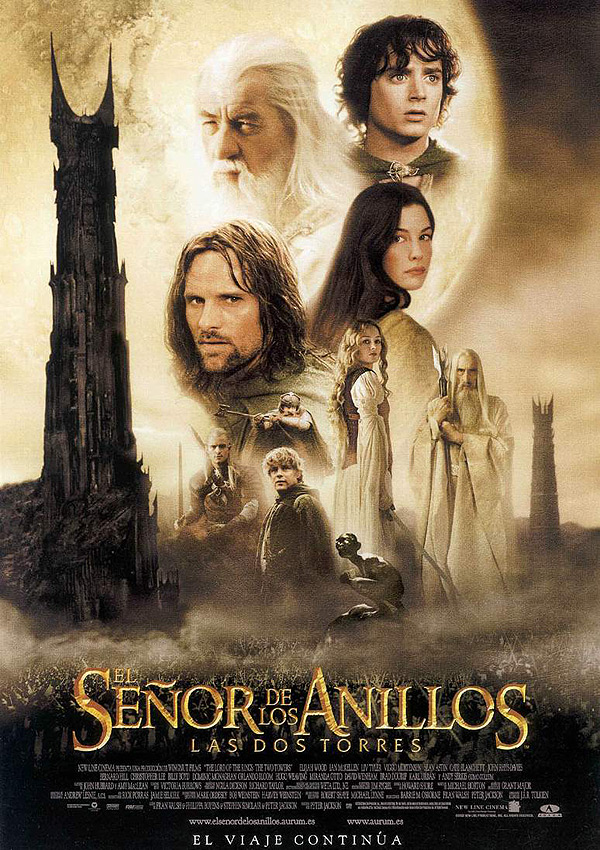
\includegraphics[scale=0.5]{IMG/13.jpg}
\caption {Adjunto imagen de una portada}

\label{fig:anillos}
\end{figure}

Podemos ver una portada de una de las \emph{películas} en la \emph{\textbf{Figura}}~\ref{fig:anillo}


